\documentclass[showpacs, oneside, onecolumn, prl, amsmath, amssymb, nofootinbib, superscriptaddress, notitlepage]{revtex4-1}


\usepackage{cases}
\usepackage{amsmath}
\usepackage{amssymb}
\usepackage{amsfonts}
\usepackage{amssymb}
\usepackage{dcolumn}
\usepackage{bm}
\usepackage{bbm}
\usepackage{graphicx}
\usepackage{xcolor}
\usepackage{array}
\usepackage{subfigure}
\usepackage{hyperref}
\usepackage{multirow}
\usepackage{ulem}

%%%%%%%%%%%%%%%%%%%%%%%%%%%%%%%%%%%%%%%%%%%%%%%%%%%%%%%%%%%%%%%%%%%%%%%%%%%%%%%%%%%
\newcommand{\bra}[1]{\langle #1\vert}
\newcommand{\ket}[1]{\vert #1\rangle}
\newcommand{\nn}{\nonumber \\}
\newcommand{\lag}{\langle}
\newcommand{\rag}{\rangle}
\newcommand{\cN}{{\cal N}}
\newcommand{\cA}{{\cal A}}
\newcommand{\gsim}{\mathrel{\hbox{\rlap{\lower.55ex \hbox {$\sim$}}
                   \kern-.3em \raise.4ex \hbox{$>$}}}}
\newcommand{\lsim}{\mathrel{\hbox{\rlap{\lower.55ex \hbox {$\sim$}}
                   \kern-.3em \raise.4ex \hbox{$<$}}}}

\newcommand\be{\begin{equation}}
\newcommand\ba{\begin{align}}
\newcommand\bas{\begin{align*}}
\newcommand\bt{\begin{table}}
\newcommand\bts{\begin{table*}}
\newcommand\bfig{\begin{figure}}
\newcommand\bfs{\begin{figure*}}
\newcommand\ee{\end{equation}}
\newcommand\ea{\end{align}}
\newcommand\et{\end{table}}
\newcommand\ets{\end{table*}}
\newcommand\efig{\end{figure}}
\newcommand\efs{\end{figure*}}
\newcommand\RA{$\ \ \Rightarrow\ \ $}
\newcommand\MC{\mathcal}
\newcommand\MBF{\mathbf}
\newcommand\MBB{\mathbb}

\newcommand\blue{\textcolor{blue}}
\newcommand\gray{\textcolor{gray}}
\newcommand\green{\textcolor{teal}}
\newcommand\red{\textcolor{red}}




\hypersetup{colorlinks=true,
            breaklinks=true,
            pdfstartview=Fit,
            linkcolor=blue,
            citecolor=green,
            urlcolor=blue}

\bibliographystyle{apsrev4-1}




%%%%%%%%%%%%%%%%%%%%%%%%%%%%%%%%%%%%%%%%%%%%%%%%%%%%%%%%%%%%%%%%%%%%%%%%%%%%%%%%%%%
\begin{document}
	
\title{Final Project For N-Body}

\author{JIAO Hao ~~ 260955982}

\maketitle

~~~~

I finish this final project in one python file \textbf{``JIAO Hao\_project.py''}, and I set a variable named ``Part'' corresponding to running the code of whichpart at the begining of this file.

~~~~

\textbf{Parameters:}

For most parts (default mode), I set the number of grids is \textbf{125} on every axes ($125^3=1.9\times10^6$ cells).

I set \textbf{the size of each cell is 1}, so it is easy to get the coordinate of every particles:
\be
pos\_x=int(x)
\ee
The way to change the size to any other value is shown in the py file and denoted by double quotation marks (line 19-33). I know this because at first, I use that formalism (pos\_min, pos\_max \& ngrid), but then, I found that it is much more concise to set the length =1.

~~~

Besides, since for most cases, the number of particles is much smaller than the number of cells, I set the force in ``class particles'' is corresponding to every particles rather than every grid cells.

~~~~

Since I show the evolution of particles for every part by gif figure, I cannot show them in this file. I will point out which file corresponding to which part in this file.

~~~~

~~~~

%%%%%%%%%%%%%%%%%%%%%%%%%%%%%%%%%%%%%%%%%%%%%%%%%%%%%%%%%%%%%%%%%%%%%%%%%%%%%%%%%%%
\section{Part 1 One rest particle}

~~~~

Here I simply talk about my main idea of this project (except for some detail corresponding to other parts):

~~~~

\textbf{The Green function}: I first tried to use Conjugate Gradient to solve the green function, but find it isn't very precise. So I directly use the expression of the green function of 3D gratitational potential (refer to the professor's file ``laplace\_fft.py''). And since we set Green[0,0,0] to be a finite number, we automatically soften the potential.

In order not to calculate the Green function every step, I first get the variable named Green (just for the periodic case).

The non-periodic case is mentioned on part 3.

~~~~

\textbf{Get the potenial}: For periodic case, I can directly get the potential by convoluting the density of particles and Green function with the same size of our space ($125\times125\times125$).

I use ``np.fft.ftt'' rather than ``np.fft.rfft'' because I set the ngrid to be odd and will have problem with ``np.fft.rfft'' (shape will change after irfft). So I need only use the real part of potential (I have check that the image part is much smaller than the real part).

~~~~

\textbf{Get force}: The force of every particle is set to be the force at the center of the grid cell where it is. This is because we don't want it's self-gravity affects it's movement, but at the same time, the particles in the same grid cell cannot attrat it as well (another soften).

The periodic boundary condition is also shown here: the particles at boundary can fell the force from the other sides.

~~~~

\textbf{Evolve}: I use the leapfrog solver to get the evolution of every particles. The boundary condition affects the evolution twice every step.

The function `outside` is to deal with the effects of periodic/non-periodic BC when evolving. For periodic case, the particel will move to another side if it is out of one side.

~~~~

~~~~

\textbf{The evolution of an initail rest single particle}:

The result is shown in \textbf{``JH\_1.gif''}

Here we should set the number of particle npart=1, and the type is `random'(default mode). So we can get a rest particle at a random place in the grid. And the result show that it will keep rest at any time.

I set the time at the right top of the figure.

~~~~

~~~~

%%%%%%%%%%%%%%%%%%%%%%%%%%%%%%%%%%%%%%%%%%%%%%%%%%%%%%%%%%%%%%%%%%%%%%%%%%%%%%%%%%%
\section{Part 2 A pair of particles in a circular orbit}

The result is shown in \textbf{``JH\_2.gif''}

Here we should choose the ``type=`circular''' and in that type, I set the two particle initially at $(\pm \text{ngrid}/10,0,0)$ around the center of the grid. And the initial velocity is given by the circular motion:
\bas
f=\frac{Gm_1m_2}{|r_1-r_2|^2}=\frac{m_1v_1^2}{|r_1-r_2|/2}\ \ \Rightarrow\ \ v_1=\sqrt{\frac{Gm_2}{2|r_1-r_2|}}
\end{align*}

From these initial conditions, I get very precise circular orbit: with error (of the length of radius) less than $3\%$.

\textit{Sorry that I set the track of the green particle (light green line) above the blue particle so the figure at late time is not very beautiful, but this won't affect the result and this code took dozens of hours (in my laptop) so I didn't run it again.}

~~~~

~~~~

%%%%%%%%%%%%%%%%%%%%%%%%%%%%%%%%%%%%%%%%%%%%%%%%%%%%%%%%%%%%%%%%%%%%%%%%%%%%%%%%%%%
\section{Part 3 Many particles with periodic and non-periodic boundary conditions}

The evolutions are shown in \textbf{``JH\_3\_peri.gif''} and \textbf{``JH\_3\_nonperi.gif''} (and \textbf{``JH\_3\_nonperi\_bounce.gif''} for bounced boundary condtion, see below).

I set \textbf{5000 particles} in both cases.

~~~~

\textbf{Periodic case}: The evolution of the particles are as expect:

The particles firstly collapse into many small clusters (and rotate around the center) and these clusters generally merger into a big cluster (relaxation). After this, the energy of this system tend to flat (virialization).
\newline(\textbf{JH\_3\_peri.gif})

%------
\bfig
	\centering
	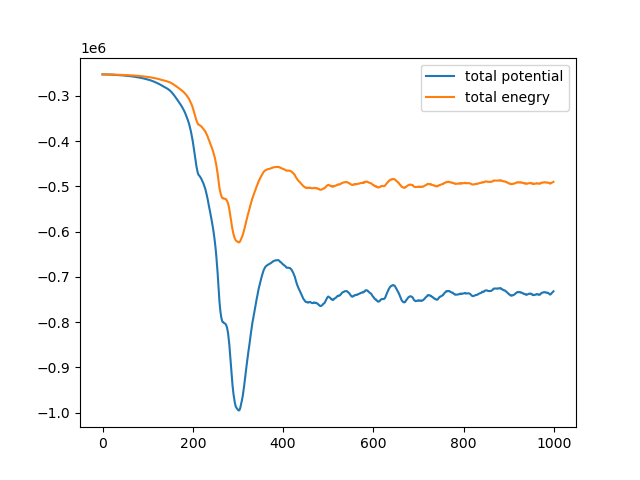
\includegraphics[scale=1]{JH_3_peri_energy.png}
	\caption{Evolution of the energy of the system of 5000 particles in a periodic box. The time interval here is 0.1 second (unit of horizontal axis).}
	\label{3-peri-energy}
\efig

I show the evolution of the potenial energy and total energy of this system in fig.\ref{3-peri-energy}(\textbf{JH\_3\_peri\_energy.png}) and we can find that after 50s, the two energies become approximately constant. But the potential energy is not exactly the twice of the total energy, I think this is because our potential may not the real gravitational potential (=0 at infinity), we can solve this by adding a suitable offset. The fluctuations of total enegry in this period is also approximately half of that of potential energy.


~~~~

\textbf{Non-preriodic case}: 

~~~~
\textbf{The Green's function and potential}: I set the Green function in a box with each side twice the length of the box in order to get rid of the effect of the other side (total scale $[ngrid+2*(ngrid//2),ngrid+2*(ngrid//2),ngrid+2*(ngrid//2)]$). \newline
Because of this, the calculation amount is much larger than periodic case, I only set \textbf{ngrid=75} here.

\gray{At first, (in order to not convolute in a nearly 7 times larger box) I try to use Conjugate Gradient to get the potential of every steps, but find that this method is much slower and very imprecise.\newline I didn't try to input the present potential to get the potential of next step, this method might work.}

Besides, to get the force at an edge of the box, I preserve the potential of a grid with one more cell on each sides (total scale $[ngrid+2,ngrid+2,ngrid+2]$). This also show in the function ``get\_force''.


~~~~

About what happens when particle move outside the box, I want to consider 2 cases:

\textbf{(i)} the particles will disappear once move outside the edges of box:\newline
I show this in the function ``outside(self,periodic=True)'' (around line 222) with the variable ``disappear=True''. I need to change the number of particles twice every step (due to leapfrog). And I set once the number of particle less than 1000 (1/5 of the total particles), the evolution will stop.

In this case, the particles will direct collapse into one large cluster (the particles near vertex will collapse slower due to smaller force exerted on them). And then, this compact cluster will go outside this box.\newline
(\textbf{JH\_3\_nonperi.gif})

But I don't know why the main part of the cluster will move to one vertex of the box.

%------
\bfig
	\centering
	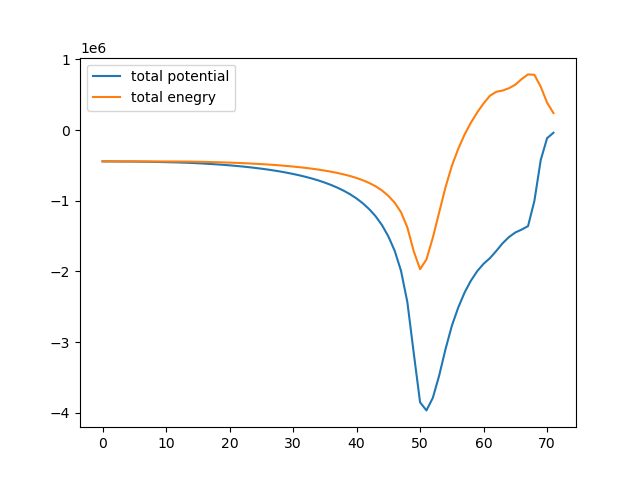
\includegraphics[scale=0.8]{JH_3_nonperi_energy.png}
	\caption{Evolution of the energy of the system of 5000 particles in a non-periodic box, assuming that particles disappear once move outside the box. The time interval here is 0.1 second (unit of horizontal axis).}
	\label{3-nonperi-energy}
\efig

%------
\bfig
	\centering
	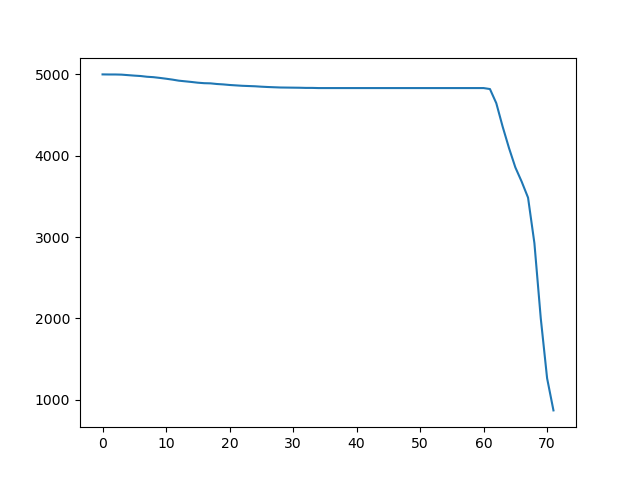
\includegraphics[scale=0.8]{JH_3_nonperi_particlenumber.png}
	\caption{Evolution of the number of particles of the system with 5000 particles at beginning in a non-periodic box, assuming that particles disappear once moving outside the box. The time interval here is 0.1 second (unit of horizontal axis).}
	\label{3-nonperi-number}
\efig


This system doesn't relaxed/virialized, so the total/potential energy won't converge at all. It is show in fig.\ref{3-nonperi-energy} (\textbf{JH\_3\_nonperi\_energy.png})

The number of particles: At first, a little amount of particles move out of the box, and then the number conserved during collapsing since they all move towards the center. After that, the number of particles decrease rapidly. See fig.\ref{3-nonperi-number} (\textbf{JH\_3\_nonperi\_particlenumber.png})

~~~~

\textbf{(ii)} the particles will bounce back when moving outside the edges of box:\newline
The main difference is in the function ``outside'', where in this case, I set ``disappear=False''.\newline
(\textbf{JH\_3\_nonperi\_bounce.gif})

This boundary condition does not change the evolution of the system a lot before the end of collapse, but after that, the cluster will biunce back from the vertex. So this case is not important. The total enregy is not conserved since we ignore the potential energy outside the box.


~~~~

~~~~

%%%%%%%%%%%%%%%%%%%%%%%%%%%%%%%%%%%%%%%%%%%%%%%%%%%%%%%%%%%%%%%%%%%%%%%%%%%%%%%%%%%
\section{Part 4 the universe with a scale-invariant power spectrum}

The evolutions of this part are shown in files named like \textbf{``JH\_4\_n=xxxx.gif''}

I try several different number of particles here, and still use \textbf{ngrid=125} for the first 3 cases (\textbf{n=5000,20000 and 100000}). But the last case I set \textbf{n=420k} with \textbf{ngrid=75} so there isapproximately 1 particle per cell on average.

~~~~

The initial density distrubution on every grid is defined in ``density\_part4(ngrid)'':\newline
I get a white noise on the grid in real space and trasform to Fourier space and times $\sqrt{P(k)}=k^{-3/2}$ to get the density distriibution in Fourier space (den\_ft). I set dens\_ft[0,0,0]=0, and transform it to real space. We only need the real part of this density distribution and I have checked that the image part of this is much smaller than the real part. Then I add a offset to the density distribtion to make sure it is positive and normalize it.\newline
Indeed, in real life, the fluctuation should much smaller than the average density, but for simplification, I just set as above.

I use rejection method to get the initial distribution of partices (see function ``get\_dens\_part4(n)'')

%------
\bfig
	\centering
	\includegraphics[scale=0.8]{JH_4_density.png}
	\caption{The initial density distribution of one slide of the grid -- dens[:,:,ngrid//2].}
	\label{4-density}
\efig

A slide of the initial distribution (of one case) is show in fig.\ref{4-density} (\textbf{JH\_4\_density.png}) and I think it is reasonable.

~~~~
%------
\bfig
	\centering
	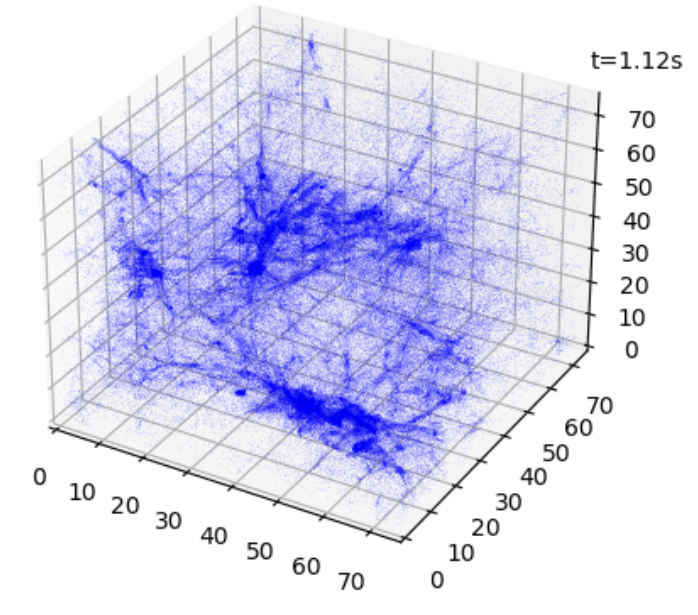
\includegraphics[scale=0.8]{JH_4_n=420000_LSS.png}
	\caption{The ``large scale structure'' during the evolution of 420k particles in a box with $75^3$ grid cells.}
	\label{4-LSS}
\efig

The evolution of this system: These particles will still eventually collapse into one big cluster, but the process is different in this case:\newline
The $k^{-3}$ initial distribution will form some ``large scale structure' (compared with the scale of small clusters) during the eventual collapse. And the more particle in the box, the LSS is more obvious. I show this in fig.\ref{4-LSS} (\textbf{JH\_4\_n=420000\_LSS.png}). We can see filaments, nodes and voids here (sorry that I am not sure if there are sheets), It is similar to our real universe.

To get better result, for different number of particles, I set different time steps and transparencies:\newline
For n=5000, ngrid=125: dt=0.05/20=0.0025, $\alpha$=0.4\newline
For n=20000, ngrid=125: dt=0.02/20=0.001, $\alpha$=0.4\newline
For n=100000, ngrid=125: dt=0.02/20=0.001, $\alpha$=0.2\newline
For n=420000, ngrid=75: dt=0.01/20=0.0005, $\alpha$=0.05, and I set m=0.4 to let the evolution not too fast.

~~~~
%------
\bfig
	\centering
	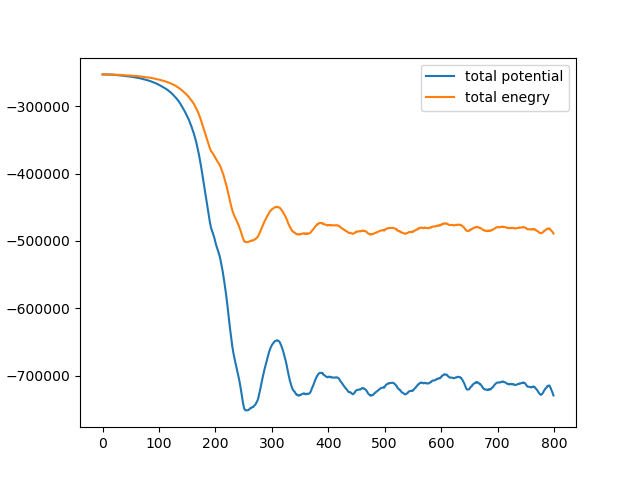
\includegraphics[scale=0.8]{JH_4_n=5000_energy.png}
	\caption{The ``large scale structure'' during the evolution of 420k particles in a box with $75^3$ grid cells.}
	\label{4-energy}
\efig

Since in this part, we are not required to track the total energy, I only plot the total energy for n=5000 case, shown in fig\ref{4-energy}. And we can see that it's also conserved after relaxation.





\end{document}